\documentclass{article}


\usepackage{arxiv}

\usepackage[utf8]{inputenc} % allow utf-8 input
\usepackage[T1]{fontenc}    % use 8-bit T1 fonts
\usepackage{hyperref}       % hyperlinks
\usepackage{url}            % simple URL typesetting
\usepackage{booktabs}       % professional-quality tables
\usepackage{amsfonts}       % blackboard math symbols
\usepackage{nicefrac}       % compact symbols for 1/2, etc.
\usepackage{microtype}      % microtypography
\usepackage{lipsum}
\usepackage{siunitx}
\usepackage[linesnumbered,ruled,vlined]{algorithm2e}
\usepackage{float}
\usepackage{amsmath}
\usepackage{enumerate}
\usepackage{cite}
\usepackage{xcolor}
\usepackage{graphicx}
\graphicspath{ {../img/} }

\newcommand{\note}[1]{\textbf{#1}}

\title{Your EA Report Title}


\author{
 Xiang He\\
  s3627136\\
  \texttt{1234@umail.leidenuniv.nl}\\
  %% examples of more authors
   \And
 Shupei Li\\
  s3430863\\
  \texttt{s.li.18@umail.leidenuniv.nl} \\
  %% \And
 %% Name \\
  %% Student number\\
  %% \texttt{email address} \\
  %% \AND
  %% Coauthor \\
  %% Affiliation \\
  %% Address \\
  %% \texttt{email} \\
  %% \And
  %% Coauthor \\
  %% Affiliation \\
  %% Address \\
  %% \texttt{email} \\
  %% \And
  %% Coauthor \\
  %% Affiliation \\
  %% Address \\
  %% \texttt{email} \\
}

\begin{document}
\maketitle
%% \begin{abstract}
%% Abstract of your report here.
%% \end{abstract}


% keywords can be removed
%\keywords{First keyword \and Second keyword \and More}


\section{Introduction}\label{sec:intro}

Introduction text here.

\section{Algorithms}
\label{sec:imple}

Outline of your algorithms, algorithm parameters, and settings used for those parameters. 

\begin{algorithm}[!ht]
\SetAlgoLined
\SetKwInOut{Input}{Input}\SetKwInOut{Termination}{Termination}

\Input{Population size $\mu$\\Crossover probability $p_c$ \\etc.}
\Termination{The algorithm terminates when..}
\BlankLine

Initialization\;

\For{$i=1$ \KwTo $B$}{
Selection\;
Crossover\;
Mutation\;
}
\caption{A framework of Genetic Algorithm \\\note{Please describe your genetic algorithm using this template}}\label{al:LOF}
\end{algorithm}
 
You can explain the implementation in various ways, as long as you make the clear and understandable. If you prefer to explain your algorithm in pseudo code, you could find an example (Algorithm \ref{al:LOF}). Please make sure that the algorithm and the results are reproducible from your description. \note{Note that if we cannot get the same results using the codes you submit, the PA grade is 0.} You can fix the random seed during your experiment and provide it to us so that we can avoid the different results caused by randomization. 




\section{Experimental Results}\label{sec:experi}

Description of the experiments and the results. Use the tables and figures generated from IOHanalyzer. Make sure to present your results in a way that is convenient to the reader, \textbf{do not blindly include plots of all your experiments, try to combine information in figures and tables!} 

Figure \ref{fig:example} and \ref{fig:test} show examples of how to insert your figure in the report. Please also see the captions, make sure you explain your figures properly in the captions.

\begin{figure}[!ht]
 \begin{center}    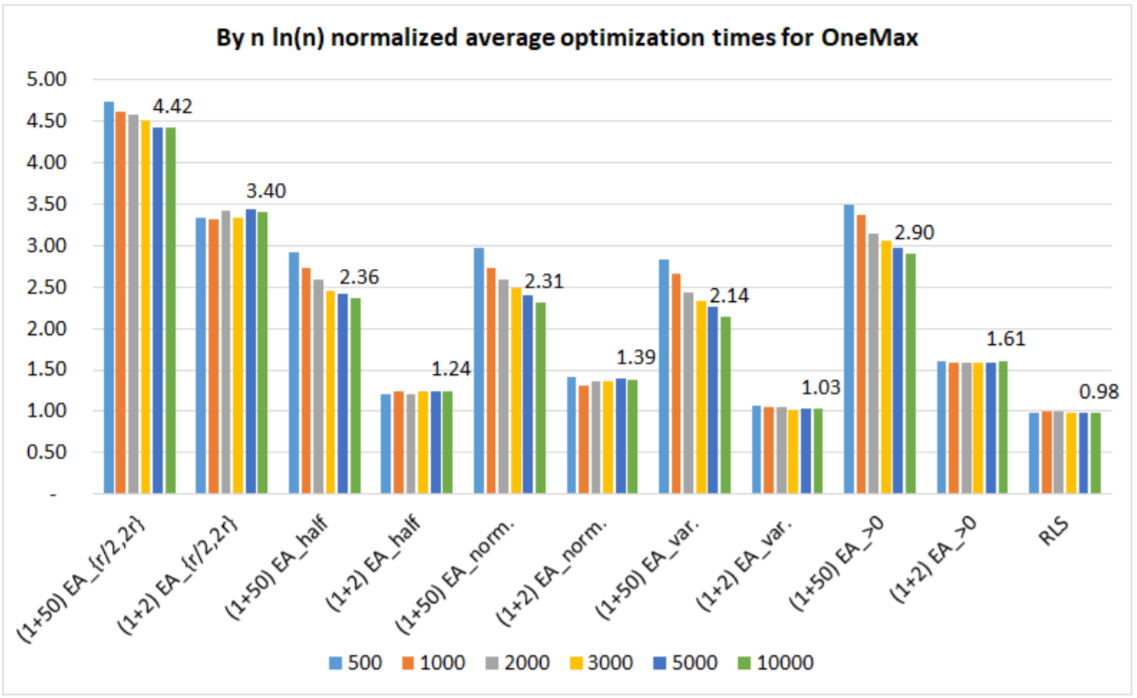
\includegraphics[width=0.95\textwidth]{example.png}
 \end{center}
 \caption{By $n\ln(n)$ normalized average optimization times for OneMax, for $n$ between 500 and 10 000. Displayed numbers are for $n = 10 000$ \cite{ye2019interpolating}.}
 \label{fig:example}
\end{figure}


\begin{figure}[!ht]
 \begin{center}    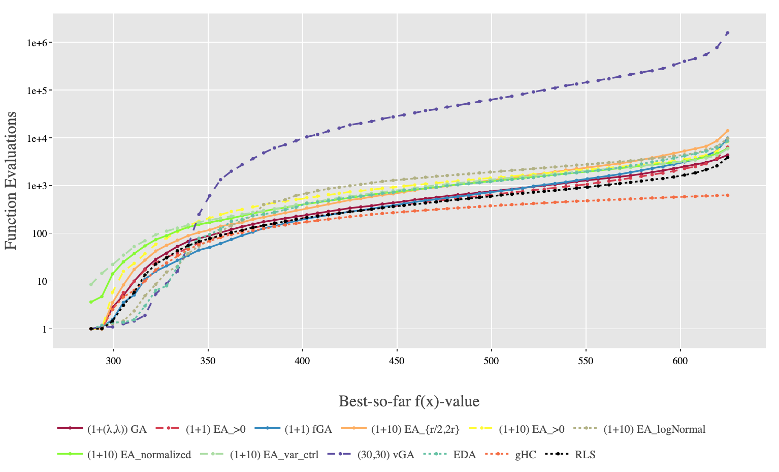
\includegraphics[width=0.95\textwidth]{best-so-far.png}
 \end{center}
 \caption{The fixed-target results of 11 algorithms. The figure is downloaded from IOHanalyzer.}
 \label{fig:test}
\end{figure}


Table \ref{tab:test} and  Table \ref{tab:test2} show two examples of how to insert your tables in the report. \note{Note that the \emph{tex} files of tables can also be downloaded from IOHanalyzer.}

\begin{table}[!ht]
 \caption{Sample table 1 title}
  \centering
  \begin{tabular}{lll}
    \toprule
    \multicolumn{2}{c}{Part}                   \\
    \cmidrule(r){1-2}
    Name     & Description     & Size ($\mu$m) \\
    \midrule
    Dendrite & Input terminal  & $\sim$100     \\
    Axon     & Output terminal & $\sim$10      \\
    Soma     & Cell body       & up to $10^6$  \\
    \bottomrule
  \end{tabular}
  \label{tab:test}
\end{table}

\begin{table}[!ht]
 \caption{Sample table 2 title}
    \centering
    \begin{tabular}{SSSSSSSS} \toprule
    {$m$} & {$\Re\{\underline{\mathfrak{X}}(m)\}$} & {$-\Im\{\underline{\mathfrak{X}}(m)\}$} & {$\mathfrak{X}(m)$} & {$\frac{\mathfrak{X}(m)}{23}$} & {$A_m$} & {$\varphi(m)\ /\ ^{\circ}$} & {$\varphi_m\ /\ ^{\circ}$} \\ \midrule
    1  & 16.128 & +8.872 & 16.128 & 1.402 & 1.373 & -146.6 & -137.6 \\
    2  & 3.442  & -2.509 & 3.442  & 0.299 & 0.343 & 133.2  & 152.4  \\
    3  & 1.826  & -0.363 & 1.826  & 0.159 & 0.119 & 168.5  & -161.1 \\
    4  & 0.993  & -0.429 & 0.993  & 0.086 & 0.08  & 25.6   & 90     \\ \midrule
    5  & 1.29   & +0.099 & 1.29   & 0.112 & 0.097 & -175.6 & -114.7 \\
    6  & 0.483  & -0.183 & 0.483  & 0.042 & 0.063 & 22.3   & 122.5  \\
    7  & 0.766  & -0.475 & 0.766  & 0.067 & 0.039 & 141.6  & -122   \\
    8  & 0.624  & +0.365 & 0.624  & 0.054 & 0.04  & -35.7  & 90     \\ \midrule
    9  & 0.641  & -0.466 & 0.641  & 0.056 & 0.045 & 133.3  & -106.3 \\
    10 & 0.45   & +0.421 & 0.45   & 0.039 & 0.034 & -69.4  & 110.9  \\
    11 & 0.598  & -0.597 & 0.598  & 0.052 & 0.025 & 92.3   & -109.3 \\ \bottomrule
    \end{tabular}
    \label{tab:test2}
\end{table}



\section{Discussion and Conclusion}\label{sec:dis&res}

Summarize the results and conclude your report. If you would like to put main conclusions  discussions as lists in this part, you can see an example below.

\begin{enumerate}[1)]
    \item We suggest using population size $\mu=x$ for the genetic algorithm solving the problem.
    
    \item The genetic algorithm benefits from small mutation rates as solving the \textsc{NAS} problem. (Just an example, this may not be not the truth.)
    
    \item We observe that the evolution strategy benefits from comma selection for solving the \textsc{NAS} problem. (Again, just an example).
\end{enumerate}
 
 \textbf{Tips:} Please put the references in the file \emph{references.bib} and cite them in the right line, like this \cite{hadash2018estimate}.

\bibliographystyle{unsrt}  
\bibliography{references}  




\end{document}
